%\textbf{Problem statement: } \textit{Write a pass that counts the number of static instructions in a program.} \\
%\textbf{Problem instance:} \textit{Output for each instruction the number of times it appears in the program.}
\subsection{Pass Algorithm description}

Because the functionality is a static analysis, it is sufficient to run a pass on the compiled code of each benchmark.
We store instruction op codes and their corresponding count in a C++ map structure. Each time an instruction is found in the source code, it is either added to an existing map entry or a new entry is created and initialized to 1.

A high level algorithm description is given on algorithm 1, where :
\begin{itemize}
\item {$I$ is an input program instruction list in LLVM byte code (.bc) format}
\item{$i$ is an individual instruction within $I$}
\item{$M$ is a C++ map of the form \code{<string,int>}}
\end{itemize}

\begin{algorithm}
 \KwIn{$M$,$I$}
 $t \gets 0$\\
 \ForAll{$i \in I$}
 { 
 	\If{$M$.containsKey($i$)}
 	{
 		$M$.valueForKey($i$)+=1\\
 	}
 	\Else
 	{
 		$M$.insertKeyValuePair($<i$,$1>$)\\
 	}
 }
 \ForAll{keyValuePair $\in M$}
 {
 	print("Found "keyValuePair.value() "counts of: "keyValuePair.key())\\
 	$t$ += keyValuePair.value()\\
 }
 print("total instructions: "$t$)
 \caption{Static instruction count algorithm}
\end{algorithm}

\subsection{Physical Implementation Description}
%Besides a working proficiency in C++, translating the algorithm to LLVM required an understanding of:
%\begin{itemize}
%\item how to build and run an opt module on a target benchmark program
%\item how to output data in human readable format from an opt module
%\item how instructions are represented by LLVM
%\item how instructions are accessed by opt modules
%\end{itemize}

While the above is the abstract description of what we are trying to achieve, we have to adapt our algorithms to the syntax and semantics of an LLVM \code{opt} pass framework. The general purpose of an \code{opt} pass is to instrument an input bitcode file and ouptut its instrumentation. This process is done using different C++ classes (and methods) depending on the scope of the instrumentation. We chose to use the \code{ModulePass} class (and \code{RunOnModule(Module \&M)} method) which gives us simultaneous access to all the functions in the input file, make are counting task easier. \\

In order to represent the $\textbf{forall the } i \in I$ iteration, we use the iterator abilities of the Module and Function classes as follows :

\begin{frame}[fragile]
%\frametitle{Inserting source code}
\lstset{language=C++,
                basicstyle=\ttfamily,
                keywordstyle=\color{blue}\ttfamily,
                stringstyle=\color{red}\ttfamily,
                commentstyle=\color{green}\ttfamily,
                morecomment=[l][\color{magenta}]{\#}
}
\begin{lstlisting}
for (Module::iterator m = M.begin(),
    e = M.end() ; e != m ; ++m) {
    for (inst_iterator I = 
    inst_begin(m), E = inst_end(m) ;
    I != E ; ++I) {...}
\end{lstlisting}
\end{frame}

The body of the algorithm (lines 3 to 6) could then be implemented using standard C++. Finally, to output the results of our analysis we implemented the \code{void print(raw\_ostream \&OS, const Module\*) const} function which allows use to print out our analysis result using the \code{-analyze} flag of the \code{opt} module. 

%\begin{frame}[fragile]
%\frametitle{Inserting source code}
%\lstset{language=C++,
%    basicstyle=\ttfamily,
%    keywordstyle=\bfseries,
%    showstringspaces=false,
%    morekeywords={runOnModule}                
%}
%\begin{lstlisting}
%    virtual bool runOnModule(Module &M)()
%\end{lstlisting}
%\end{frame}

%Accessing instructions was accomplished by iterating through the \textbf{input source} \textbf{Module} using an \textbf{inst\_iterator}. The Module contains all instructions from the compiled benchmark and the inst\_iterator points at individual instructions.\\


\subsection{Benchmark analysis}
We analysed module performance by comparing the logged instruction count with manual and automatic counts of the intermediate .ll byte code of each compiled benchmark. The automated counts were performed with the grep command
\code{cat [benchmark-name.ll] | grep [instruction-name] -c}. The counts were accurate, confirming the pass' correct functionality.
%\begin{figure}[here]
%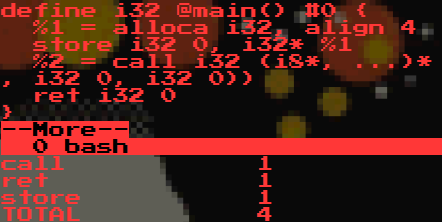
\includegraphics[width=0.4\textwidth]{StaticInst}
%\caption{Example correct pass output}
%\label{StaticInstCount}
%\end{figure}